\section{Infraestrutura}

\subsection{Arquitetura}

Em seguida é apresentada a arquitetura da infraestrutura escolhida.

--- IMAGEM

\subsection{Storage}
Esta componente é responsável por garantir alta disponibilidade e lidar com a persistência, quer nas máquinas, quer nos discos que a compõem. Tendo em conta o dito anteriormente optou-se por colocar dois discos para persistência de dados do website, e outros dois discos para armazenar a base de dados PostgreSQL. Para lidar com cada par de discos despenderam-se duas máquinas que contem os serviços DRBD e iSCSI. O primeiro serviço simula dois RAID1, onde a caracteristica é a replicação de dados, que no futuro, além da disponibilidade em caso de falha, torna-se bastante útil nas laeituras de disco. O segundo serviço é responsavel por permitir o acesso estes discos remotamente, através de TCP/IP, que usufrui do armazenamento de dados que o serviço anterior oferece.

\subsection{Cluster}
O Service Cluter é uma componente essencial nesta infraestrutura devido à garantia que fornece quanto à alta disponibilidade. Este Cluster é composto por dois serviços, o PostgreSQL e NFS Server garantindo assim a disponibilidade inicialmente em duas máquinas e em caso de alguma falhar, então os serviçoes vão correr em apenas uma das máquinas, o que certamente irá reduzir o nivel de desempenho, mas sem nunca perder o serviço, visto que se pode agir quando o cluster manager informar que tal aconteciemento se sucedeu.

\subsection{WEB}
Esta componente apenas vai receber e atender os pedidos que chegam do exterior, ou seja, contêm o serviço httpd para interpretar os pedidos e o NFS Cliente, que se conecta ao NFS Server do Cluster, onde terá acesso aos ficheiros que necessita para a interpretação e resposta do pedido.

\subsection{LVS}
Para garantir que a infraestrutura é estável e segura, foi necessário usar algo que fizesse a distribuição de carga pelos servidores da componente Web. Tendo isto em conta, foi decidido incluir duas máquinas com serviços responsáveis por saberem para onde enviar os pedidos. Para além da distribuição de carga que estes servidores conseguem efetuar, protegem ainda a infraestrutura do mundo exterior, nomeadamente através de Virtual IP, por onde os clientes acedem ao serviço que a infraestrutura dispõe. Desta forma os servidores funcionam tambem como uma Firewall, onde são filtrados os pedidos que não são esperados pela infraestrutura, atribuindo assim, a segurança falada.
O balanceador de carga fica entre o utlziador e os servidores Web Apache de back-end que mantêm o mesmo conteúdo. Se um deles está em baixo, todos os pedidos serão automaticamente redirecionados para o servidor backend restante. o que significa que os utilizadores não notarão qualquer interrupção do serviço.

\subsection{Configurações}

\subsection{Storage}

\subsection{Cluster}

\subsection{WEB}

\subsection{LVS}
O pretendido é ter um balanceador de carga, onde a máquina irá analisar todos os servidores web definindo qual estará disponivel para dar resposta ao pedido efetuado.
A infraestrutura for pensada de forma redundante para que no caso de falha de um deles, o outro possa continuar a interpretar os pedidos, e sendo assim os utilizadores obtêm sempre uma resposta aos seus pedidos.

\subsection{Ambiente de Testes}

-- Não sei se é assim ou não
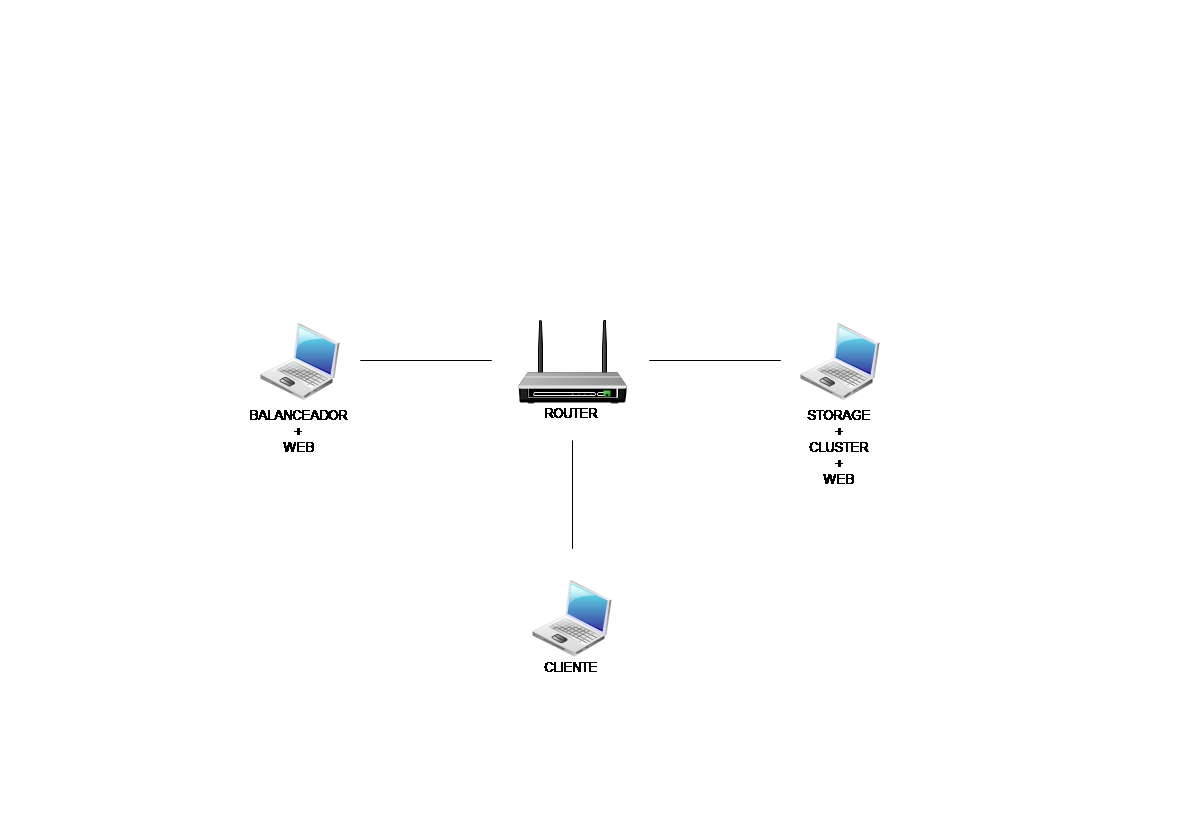
\includegraphics[scale=.4]{img/AmbienteDeTestes}

\subsection{Testes realizados e análise}

